\documentclass[a4papter]{article}
\usepackage[a4paper,bindingoffset=0.2in,%
left=1in,right=1in,top=1in,bottom=1in,%
footskip=.25in]{geometry}
\usepackage{amsmath}
%opening
\usepackage{tikz}
\usetikzlibrary{arrows}

\tikzset{
	treenode/.style = {align=center, inner sep=0pt, text centered,
		font=\sffamily},
	arn_n/.style = {treenode, circle, black, draw=black, text width=1.5em, thick},% arbre rouge noir, noeud noir
	arn_r/.style = {treenode, circle, black, draw=black, 
		text width=1.5em, thick},% arbre rouge noir, noeud rouge
	arn_x/.style = {treenode, rectangle, draw=black,
		minimum width=0.5em, minimum height=0.5em}% arbre rouge noir, nil
}
\title{\textbf{HW8}}
\author{Kangwei Ling}        

\begin{document}
\maketitle
\section{Problems}
\begin{enumerate}
	\item A full node is a node with 2 non-null children in a binary tree. Let $F(n)$ be the \# of full nodes in a binary tree with n nodes, $L(n)$ be the \# of leaves in that tree. Show that the equation below holds for any $n > 0$.
	\begin{align*}
			F(n) = L(n) - 1
	\end{align*}
	
	\item Show the result of inserting 1, 2, 3, 4, 5, 6, 7, 8, 9, 10 into an initially empty AVL tree.

	\item 
	\begin{enumerate}
		\item 
				construct a expression tree for the expression below.
			\begin{align} \label{exp}
			x = (a + (b * c)) - ((d / e) + f)*g
			\end{align}
		\item convert Eq.\eqref{exp} to a Postfix Expression($reverse \ Polish \ notation$)
		\item convert Eq.\eqref{exp} to a Prefix Expression
			\end{enumerate}
\end{enumerate}

\section{Solution Sketch}
\begin{enumerate}
	\item We know that the \# of edges in a tree with $n$ nodes is $n-1$,
	there are two edges from every full node to its children, 0 for leaves, 1 otherwise.
	therefore,
	\begin{align*}
	2\cdot F(n) + 1\cdot(n - F(n) - L(n)) + 0\cdot L(n)= n - 1
	\end{align*}
	therefore,
	\begin{align*}
	F(n) = L(n) - 1
	\end{align*}

\item The insertion of 1, 2, 3..., 7 makes a perfect balanced AVL tree,
\begin{center}
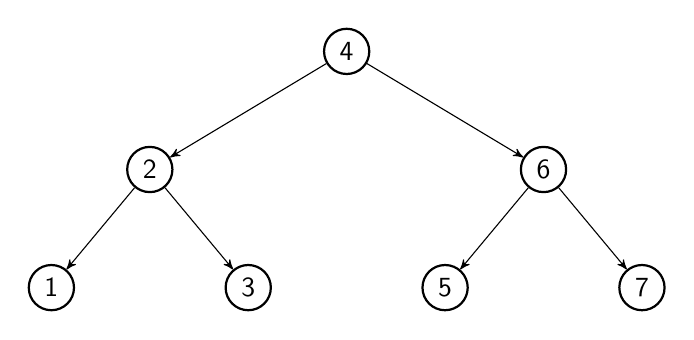
\begin{tikzpicture}[->,>=stealth',level/.style={sibling distance = 5cm/#1,
	level distance = 1.5cm}] 
\node [arn_n] {4}
child{ node [arn_n] {2} 
	child{ node [arn_n] {1} 
	}
	child{ node [arn_n] {3}
	}                            
}
child{ node [arn_r] {6}
	child{ node [arn_n] {5} 
	}
	child{ node [arn_n] {7}
	}
}
; 
\end{tikzpicture}
\end{center}
then we insert 8, 9, 10,
\begin{center}
	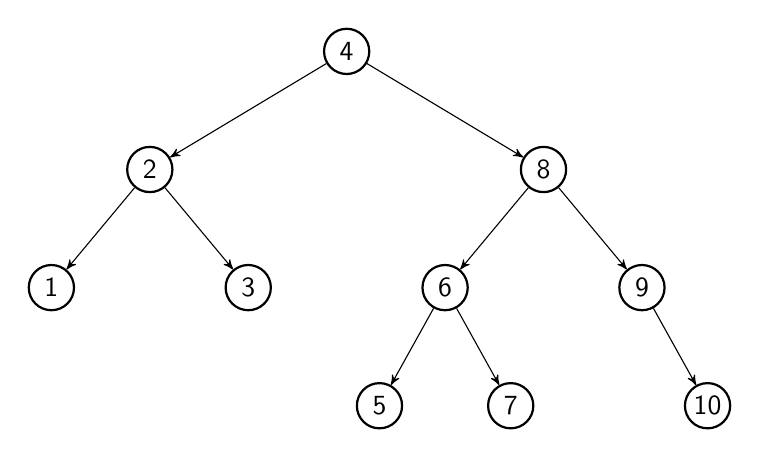
\begin{tikzpicture}[->,>=stealth',level/.style={sibling distance = 5cm/#1,
		level distance = 1.5cm}] 
	\node [arn_n] {4}
	child{ node [arn_n] {2} 
		child{ node [arn_n] {1} 
		}
		child{ node [arn_n] {3}
		}                            
	}
	child{ node [arn_r] {8}
		child{ node [arn_n] {6}
				child { node [arn_n] {5} }
				child { node [arn_n] {7} }
		}
		child{ node [arn_n] {9}
				child[missing] {}
				child {node [arn_n] {10}
		}
	}
	}
	; 
	\end{tikzpicture}
\end{center}

\item 
	\begin{enumerate}
		\item 
	Just construct the expression tree.
\begin{center}
	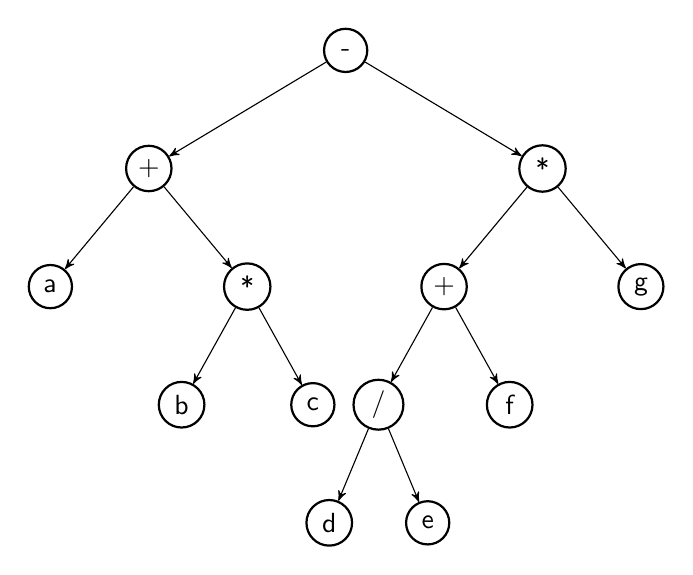
\begin{tikzpicture}[->,>=stealth',level/.style={sibling distance = 5cm/#1,
		level distance = 1.5cm}] 
\node [arn_n] {-}
		child{ node [arn_n] {+} 
				child{ node [arn_n] {a}}
				child{ node [arn_n] {*}
						child{node [arn_n] {b}}
						child{node [arn_n] {c}
							}
						}
				} 
		child{ node [arn_r] {*}
				child{ node [arn_n] {+}
						child { node [arn_n] {/} 
								child{ node [arn_n] {d}}
								child{ node [arn_n] {e}}
								}
						child { node [arn_n] {f}}
						}
				child{ node [arn_n] {g}}
				}
	; 
	\end{tikzpicture}
\end{center}

 \item Use the tree above, traverse the tree in post order.
	 \begin{align*}
	 abc*+de/f+g*-
	 \end{align*}
 \item Use the tree above, traverse the tree in pre order.
	 \begin{align*}
		 -+a*bc*+/defg
	 \end{align*}
	\end{enumerate}
\end{enumerate}
\end{document}
